\documentclass[tikz]{standalone}
\usetikzlibrary{trees}
\tikzstyle{treenode} = [draw=black,thick,anchor=west]
\begin{document}
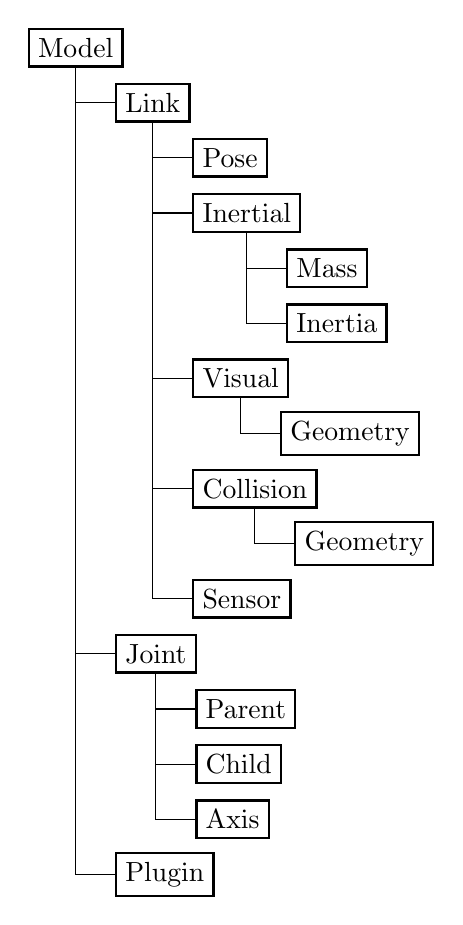
\begin{tikzpicture}[%
    grow via three points={one child at (0.5,-0.7) and two children at (0.5,-0.7) and (0.5,-1.4)},
    edge from parent path={(\tikzparentnode.south) |- (\tikzchildnode.west)}]
  \node[treenode]  {Model}
  child { node[treenode] {Link}
      child { node[treenode] {Pose} }
      child { node[treenode] {Inertial}
          child { node[treenode] {Mass} }
          child { node[treenode] {Inertia} }
        }
      child [missing] { }
      child [missing] { }
      child { node[treenode] { Visual }
          child { node[treenode] {Geometry} }
        }
      child [missing] { }
      child { node[treenode] { Collision }
          child { node[treenode] {Geometry} }
        }
      child [missing] { }
      child { node[treenode] { Sensor } }
    }
  child [missing] { }
  child [missing] { }
  child [missing] { }
  child [missing] { }
  child [missing] { }
  child [missing] { }
  child [missing] { }
  child [missing] { }
  child [missing] { }
  child { node[treenode] { Joint }
      child { node[treenode] { Parent } }
      child { node[treenode] { Child } }
      child { node[treenode] { Axis } }
    }
  child [missing] { }
  child [missing] { }
  child [missing] { }
  child { node[treenode] { Plugin } };
\end{tikzpicture}
\end{document}
